\chapter{Background}

In this chapter, we will discuss the backgrounds of the transformation that should be developed. We will start with JIAC (the target of the transformation), BPMN (the model that is being used), followed by VSDT (the existing modeling and transformation framework to JIAC that should be extended), and JET (the technology that will help us to implement the transformation).

%======================================%
%                JIAC                  %
%======================================
\section{JIAC(Java-based Intelligent Agent Componentware)}
JIAC is a Java-based agent architecture and framework that was developed to simplify the development of software agents. The framework supports the entire software development process of a software agent system by providing features such as FIPA compliant communication, Believe-Desire-Intention (BDI) reasoning, strong migration, web-service
connectivity and many others. It also provides high security (Common Criteria EAL3,
certified by the Federal Office for Information Security of Germany, BSI) and advanced
accounting mechanisms, making it suitable for the use in industrial and
commercial applications.\\

\textbf{JADL}\\
With it's core component JADL(\textit{Jiac Agent Description Language}), Jiac also provide an agent programming language. With JADL, the agents \textit{plan elements, rules, ontologies} and \textit{services} can be described. JADL is based on three predicate logic which allows the values \textit{true, false and unknown}, which makes it suitable for open world problems in unknown environments.
\\

In Figure \ref{fig:jiac_basic}, we can see the typical structure of a JIAC Application, which consists of AgentNodes, Agents, AgentBeans.
\begin{figure}[h]
	\centering
		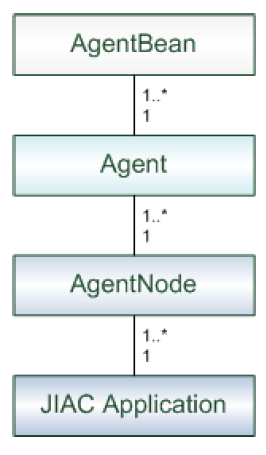
\includegraphics[width=0.25\textwidth]{images/jiac_basic.png}
		\caption{Jiac Basic concepts and their structural relationships \cite{JIACMAN10}}
	\label{fig:jiac_basic}
\end{figure}
An \textit{AgentNode} is a Java VM where the runtime infrastructure for agents, such as discovery services, white and yellow pages services, as well as communication infrastructure, are provided. A JIAC application might consists of multiple AgentNodes (distributed application). With the so-called AgentNodeBeans, one can extend the AgentNode with additional components.\\

Each AgentNode may run several \textit{Agents}. Agents provide services to other agents
and comprise lifecycle, execution cycle and a memory. An agent can use infrastructure
services in order to find other agents, to communicate to them and to use their services.
Skills and abilities of the agent can be extended by so-called AgentBeans.\\
\textit{AgentBean} is the mean to implement the functionality of an Agent, in other words, the abilities of an Agent are defined in the AgentBeans attached to it. They are plugged into agents and provide services (so-called Actions) to other agents. 


%======================================%
%                BPMN                  %
%======================================%
\section{BPMN(Business Process Modelling Notation)}
BPMN \cite{BPMN2} is a standard Notation for modelling business processes, initially published by the BPMI which is later adopted by the OMG(Object Management Group). A business process diagramm (as seen in Figure \ref{fig:bpmn_sampl}) can be compared to UML's activity diagram.
\begin{figure}[h]
	\centering
		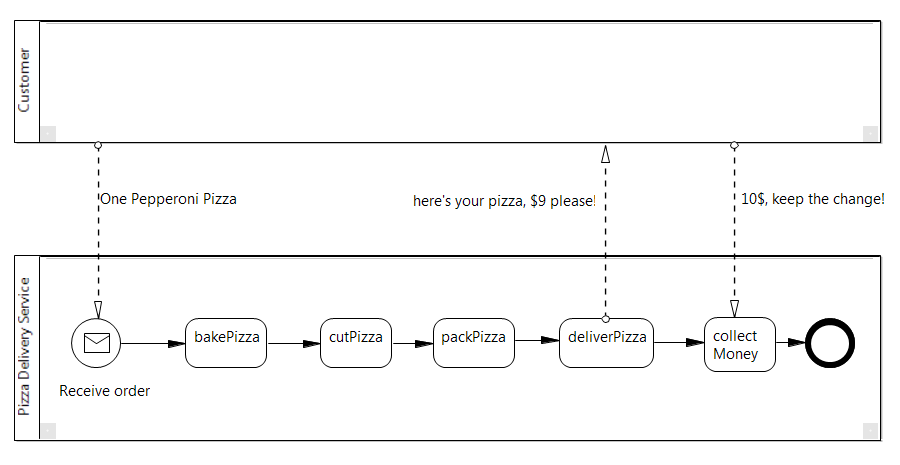
\includegraphics[width=0.90\textwidth]{images/bpmn_sampl.png}
	\caption{A simple Business Process Diagramm}
	\label{fig:bpmn_sampl}
\end{figure}\\
BPMN was made to provide a notation that is understandable by all business users, creating a bridge for the gap between the business process design and the process implementation. Besides providing an easy to read graphical notations, each BPMN elements are also equipped with additional attributes (so called properties), which are hidden from the diagram and provides the informations needed for automated code generation. With the mapping of BPMN to Agents, we hope to be able to increase the spreading of the multi agent systems in the business world.

BPMN elements can be categorized in five basic groups of elements\cite{BPMN2} :
\begin{itemize}
	\item Flow Objects
	\item Data
	\item Connecting Objects
	\item Swimlanes
	\item Artifacts
\end{itemize}
\textit{Flow Objects} includes Events, Activities and Gateways. These elements are the most important in BPMN, and they are held in a lane.\\
An \textit{Event} describes something that happens during the course of a process. It is divided into Start Event, Intermediate Event and End Event (see Figure \ref{fig:events}).
\begin{figure}[h]
	\centering
	
\includegraphics[width=0.25\textwidth]{images/events.png}
	\caption{BPMN Event types. From left to right: Start Event, Intermediate Event, End Event}
	\label{fig:events}
\end{figure}
\\
BPMN Events are further divided into subtypes according to the type of the event's trigger(for start and intermediate events) or result(for end events). The event figure(see Figure \ref{fig:event_subtypes}) are drawn with different icon in the middle, according to the trigger.
\begin{figure}[h]
	\centering
	\label{fig:event_subtypes}
	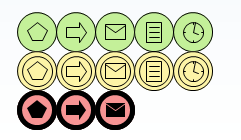
\includegraphics{images/event_types.png}
	\caption{Examples of event subtypes. From left to right: Multiple, Link, Message, Rule, Timer}
\end{figure}
%=============Add figure===============%
 
An \textit{Activity} describes something that is done during a process. It is divided into \textit{Tasks} (Atomic Activities) and \textit{Sub Processes} (Composite Activities).\\
\textit{Gateways} are used to define all kinds of splitting and merging behavior. It's semantics depends on the dimension of it's incoming and outgoing Sequence Flows.
\\\\
Data is representated by the four elements:
\begin{itemize}
	\item Data Objects
	\item Data Inputs
	\item Data Outputs
	\item Data Stores
\end{itemize}
\textit{Data Object} describes information that is needed by an activity or what they produce. It can represent a singular object or a collection of objects. \textit{Data Inputs} and \textit{Data Outputs} describe the same information for Processes. \textit{Data Stores} describe the location where information, that persists beyond the scope of a process are stored.\\\\
With \textit{ConnectingObjects}, FlowingObjects can be connected to each other or with other informations. There are 3 different kinds of Connecting Objects:
\begin{itemize}
	\item \textit{Sequence Flows} - represent Flow Control, used for connecting FlowObjects within a Pool in the order of execution.
	\item \textit{Message Flows} - represent Messages being exchanged exclusively between Pools.
	\item \textit{Associations} -  mainly used for documentation, in example between Flow Objects and a Text annotation.
\end{itemize}
\textit{Swimlanes} are divided into \textit{Pools} and \textit{Lanes}. Each Pool represents one Participant in the business process, while Lanes are used to partition a Pool, in example to model different Departments of an Institution. Figure 3 shows an empty Pool with 2 Lanes.
\begin{figure}[h]
	\centering
		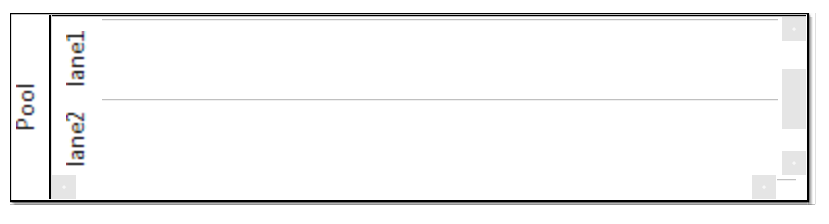
\includegraphics{images/swimlane.png}
	\caption{Empty Pool with 2 Lanes}
	\label{fig:swimlane}
\end{figure}\\\\\\
\textit{Artifacts} are additional Information about the Process. It is mainly used for documentation purpose. The Current set of Artifacts includes:
\begin{itemize}
	\item Text Annotation
	\item Group
\end{itemize}


To provide a rough overview on how Agent technology can support the implementation of Business Processes let us take a look on this mapping example of BPMN elements to Agents. A Pool in a Business Process Diagram can represent an Agent, which are able to communicate with other agents (another pool) through messages (represented with the BPMN MessageFlows). Agents can react to Events. A detailed mapping needed for implementing the transformation will be discussed in chapter \ref{chap:mapping}


%======================================%
%                VSDT                  %
%======================================%
\section{VSDT(Visual Service Design Tool)}
\label{sec:vsdt}
The VSDT is a CASE Tool, developed to support the idea of Process Oriented Agent Engineering, where Agents are designed by defining use cases and processes described with the BPMN. It's features include the BPMN editor, process structure view, model validation, import of existing web services, transformations to BPEL, and JIAC and many more. 
\begin{figure}[h]
	\centering
		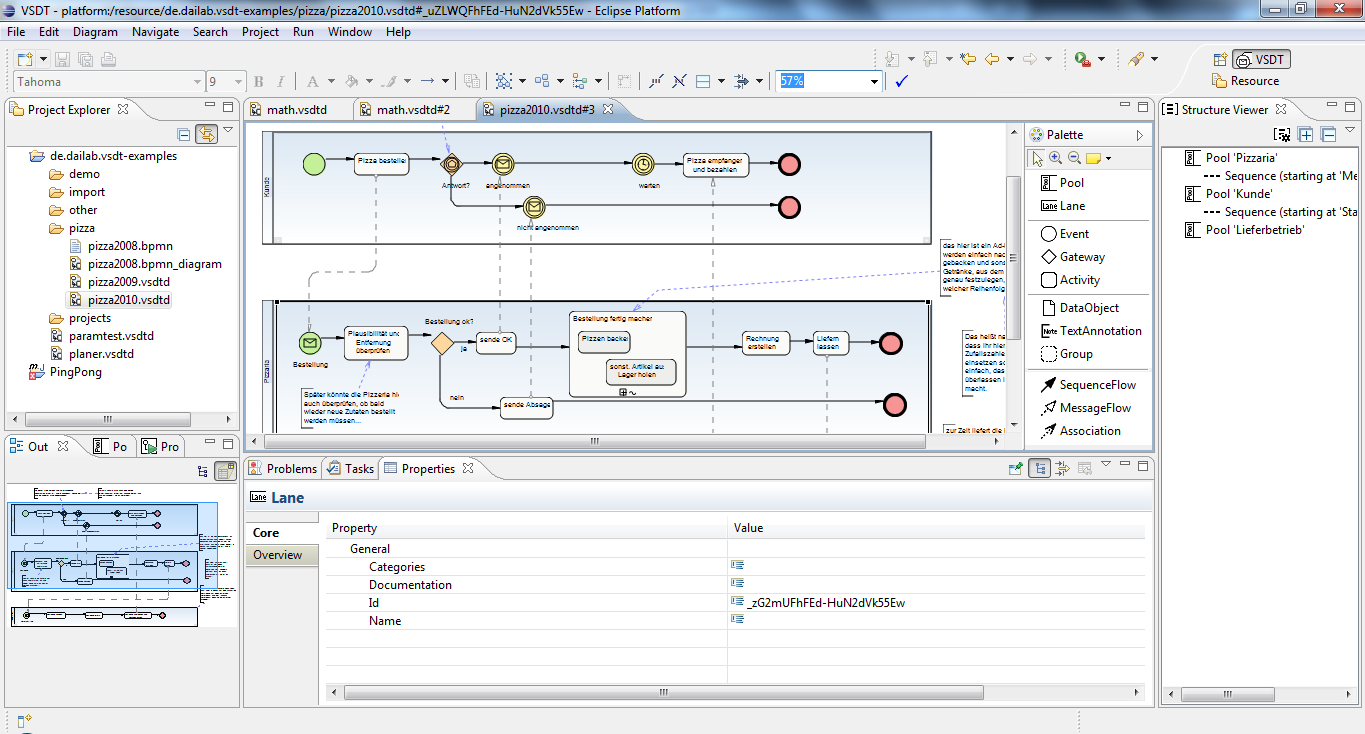
\includegraphics[width=0.90\textwidth]{images/vsdt_snapshot.png}
	\caption{VSDT - Editor View}
	\label{fig:VSDT}
\end{figure}\\

%========= The Editor =========%
\subsection{BPMN Editor}
The BPMN Editor in VSDT was created using eclipse's GMF (Graphical Modeling Framework)
%well-equipped BPMN editor that is independent of any specific target language. Thus, while the usual transformation to BPEL, as well as other transformations, is included, the VSDT can easily be extended with additional export functionality targeting other languages. It was developed in early 2007 as a Diploma Thesis at the TU Berlin and since then it has been continuously extended. 

%========= Transformation Framework ===========%
\subsection{Transformation Framework}
Since it's initial development, VSDT's transformation framework is designed to be extensible and reuseable. This allows the development of a new transformation to be easier. For this purpose the transformation process is subdivided into several stages: 
\begin{enumerate}
	\item \textit{Validation}: Validate the input model.
	\item \textit{Normalisation}: Prepare the input model for transformation.
	\item \textit{Structure Mapping}: Convert the input model to a block-like structure.
	\item \textit{Element Mapping}: Perform the actual mapping, create target model.
	\item \textit{Clean Up}: Remove redundancies, improve readability, etc.
\end{enumerate}

Due to the fact that the validation, normalisation and structure mapping are mostly independent from the target language, the standard mapping provided for these stages are reuseable, which makes it possible to implement a new transformation by specifying the element mapping only. Figure \ref{fig:transform} shows the UML Class Diagram of the transformation famework with the example transformation to BPEL.
\begin{figure}[h]
	\centering
		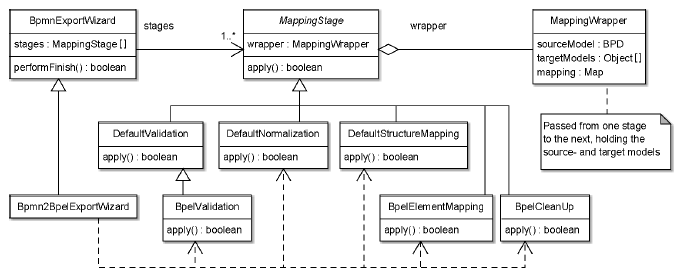
\includegraphics[width=0.90\textwidth]{images/transformation.png}
	\caption{Essential classes of the transformation framework, including the BPEL case.\cite{TK07}}
	\label{fig:transform}
\end{figure}\\

%============ Existing Transformation to Jiac ===============%
\subsection{Existing Transformation to JiacV}
At the moment, the VSDT is already equipped with a transformation of BPMN to JiacV, which generates the JADL(Jiac Agent Description Language).
The transformation to Jiac AgentBeans is in no way a replacement to the existing transformation. Instead both transformations shall complement each other as the products of both transformations have their own advantages, some of which we can find in the following table:
\begin{table}[htbp]
	\centering
		\begin{tabularx}{\linewidth}{|l|X|}\hline\hline
			\multicolumn{2}{|c|}{\textbf{Advantages of:}} \\\hline
			\multicolumn{1}{|c|}{JADL} & \multicolumn{1}{c|}{AgentBeans}\\\hline
			can be deployed to a running jiac application &  Written fully in Java, therefore developer friendly.\\
																										&  Java is more powerful that JADL.\\
			                           										&  Better performance because no parser are involved.\\\hline\hline
		\end{tabularx}
\end{table}


%======================================%
%                 JET                  %
%======================================%
\section{JET(Java Emitter Templates)}
\textit{JET}\cite{JETWEB} is a code generating framework, developed as a part of the Eclipse Modelling Project \cite{EMPWEB}. Using the so-called templates, one can transform a model into various type of text, from a simple plain text up to text containing html, xml or java code.\\\\
The transformation process is done in two steps( see figure \ref{fig:jet_process} ). First, the JET-Builder will translate the template file into a Java class holding a generate method. Then we can create an instance of the template class and call it's generate method to get the result String which we can process further for example writing it into a file. 
\begin{figure}[h]
  \label{fig:jet_process}
	\centering
		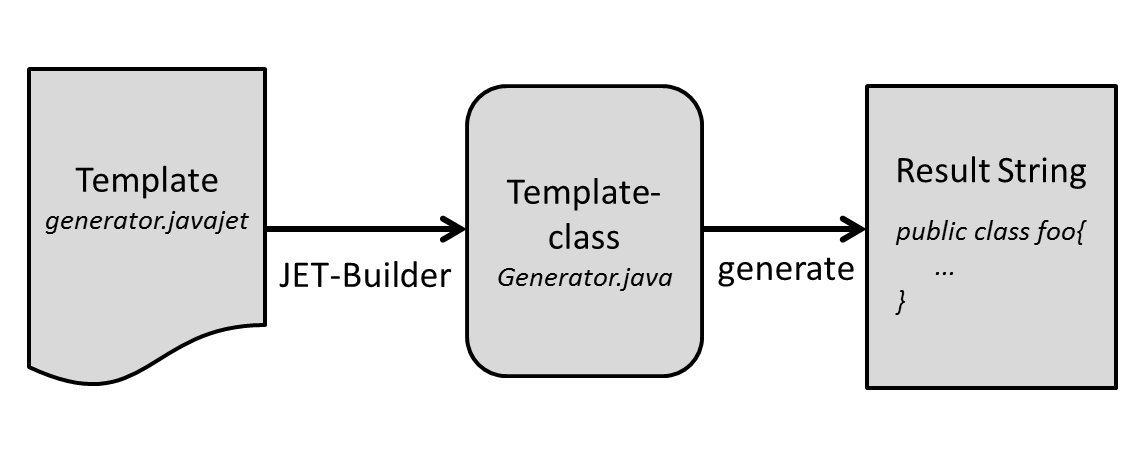
\includegraphics[width=1.0\textwidth]{images/jet_process.png}
	\caption{JET transformation steps.}
\end{figure}\\

\subsection{JET-Templates}
JET-Templates uses a JSP-like syntax which makes it easy to write and understand. The following listing shows a simple example of a JET-Template that generates an XML:
\begin{lstlisting}[caption = a simple JET-Template]
<% @ jet package="generator" imports="java.util.*" class="StudentListGenerator" %> 
<?xml version="1.0" encoding="UTF-8"?>
<% List<String> elementList = (List<String>) argument; %>
<class>
	 <% for (Iterator i = elementList.iterator(); i.hasNext(); ) { %>
     <student><%=i.next()%></student>
   <% } %>
<class>
\end{lstlisting}
A Jet-Template starts with the so called \textbf{jet-directive}. It contains informations for the JET-Builder, for example the name of the translated Java class(also called the template class), the package in which the template class should be placed into and a list of classes that should be imported by the template class.


The JET-Builder will then translate this template into the Java Class generator.StudentListGenerator:
\begin{lstlisting}[caption = the translated Java-Class, language = Java]
package generator;

import java.util.*;

public class StudentListGenerator
{
  protected static String nl;
  public static synchronized StudentListGenerator create(String lineSeparator)
  {
    nl = lineSeparator;
    StudentListGenerator result = new StudentListGenerator();
    nl = null;
    return result;
  }

  public final String NL = nl == null ? (System.getProperties().getProperty("line.separator")) : nl;
  protected final String TEXT_1 = " " + NL + "<?xml version=\"1.0\" encoding=\"UTF-8\"?>";
  protected final String TEXT_2 = NL + "<class>" + NL + "\t ";
  protected final String TEXT_3 = NL + "     <student>";
  protected final String TEXT_4 = "</student>";
  protected final String TEXT_5 = NL + "<class>";

  public String generate(Object argument)
  {
    final StringBuffer stringBuffer = new StringBuffer();
    stringBuffer.append(TEXT_1);
     List<String> elementList = (List<String>) argument; 
    stringBuffer.append(TEXT_2);
     for (Iterator i = elementList.iterator(); i.hasNext(); ) { 
    stringBuffer.append(TEXT_3);
    stringBuffer.append(i.next());
    stringBuffer.append(TEXT_4);
     } 
    stringBuffer.append(TEXT_5);
    return stringBuffer.toString();
  }
}

\end{lstlisting}


A set of JET templates is called transformation. It is possible to build this transformation with a main template which acts as a visitor and runs through the model, and this main template will then use other templates which handle a specific element of the model. For example, in UML to Java transformation you can have special templates that handles the package, class, variables and methods.\\\\

\subsection{2 different JET-Versions}\\\\
There are currently 2 different JET-Versions in the Eclipse Modelling Project. The older Version allows us to generate text with an Object as argument. In the template, one can type cast the argument variable into the class of our model. \\
The Java Class translated from the JET-Template will have the generate method: \\
\begin{lstlisting}[language=Java, caption=generate method translated from the JET-Template,
label=lst:jet_generate]
public String generate(Object argument){
	...
}
\end{lstlisting}

This JET-Version is effective if the model we want to generate the text from is a Java object. We get a String as a result which we can write into a File using the Java-IO or even Eclipse API.\\\\

In the updated version of JET, also called JET2, some workspace and java related "'tag-libraries"' are provided, enabling us to do the transformation without using the Java and Eclipse API. Unfortunately, in this Version the model has to be an xml-File.
To directly transform the BPMN directly from it's xml-Representation will be harder and the template will be confusing, therefore a decision has been made to implement the mapping using the existing transformation framework where an intermediate model class of the AgentBean will be created, and then transform this intermediate model into Java code using the older version of the JET Transformation.
More details on the implementation will be discussed in chapter \ref{chap:implementation}.